\subsection{M.PC.EAC - Estimated at Completion}
\label{sec:EAC}

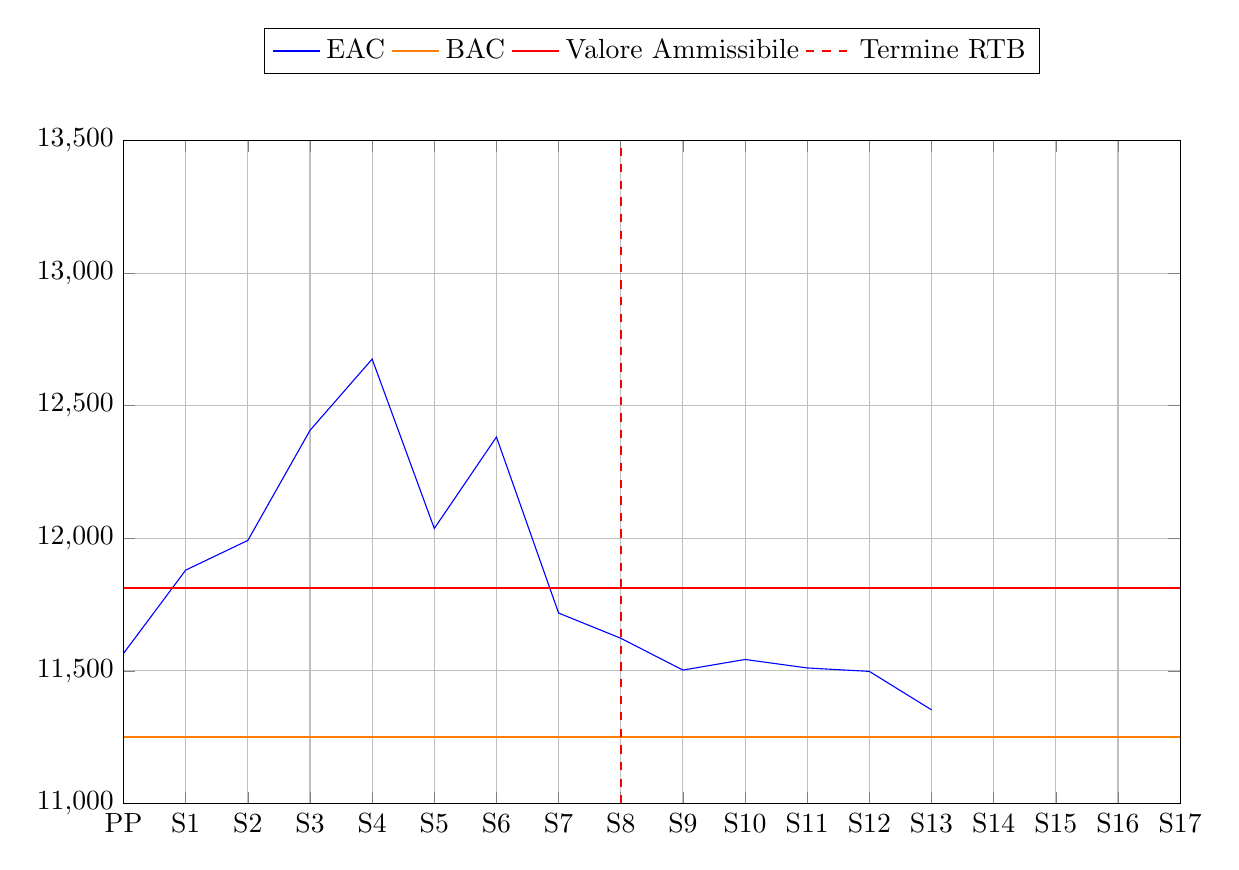
\begin{tikzpicture}
    \begin{axis}[
        width=15cm, height=10cm,
        ymin=11000, ymax=13500,
        xmin=0, xmax=17,
        xtick={0, 1, 2, 3, 4, 5, 6, 7, 8, 9, 10, 11, 12, 13, 14, 15, 16, 17, 18},
        xticklabels={PP, S1, S2, S3, S4, S5, S6, S7, S8, S9, S10, S11, S12, S13, S14, S15, S16, S17, S18},
        xlabel={},
        ylabel={},
        grid=major,
        scaled ticks=false,
        legend style={at={(0.5,1.1)}, anchor=south, legend columns=-1},
    ]
    \addplot[color=blue] coordinates {(0, 11566) (1, 11880) (2, 11992) (3, 12407) (4, 12676) (5, 12037) (6, 12382) (7, 11718) (8, 11623) (9, 11503) (10, 11543) (11, 11511) (12, 11498) (13, 11353)};
    \addlegendentry{EAC}
    \addplot[orange, thick] coordinates {(0, 11250) (17, 11250)};
    \addlegendentry{BAC}
    \addplot[red, thick] coordinates {(0, 11812.5) (17, 11812.5)};
    \addlegendentry{Valore Ammissibile}
    \addplot[red, thick, dashed] coordinates {(8, 11000) (8, 13500)};
    \addlegendentry{Termine RTB}
    \end{axis}
\end{tikzpicture}
\subsubsection{RTB}
Il grafico mostra che l'\glossario{Estimated at Completion} non risulta mai all'interno del valore ammissibile, indicando una gestione poco efficiente dei costi di progetto. 
Questo significa che il costo stimato alla fine del progetto è sempre superiore al costo preventivato. Ciò indica che c'è necessità di un'analisi più approfondita dei costi e delle attività svolte per evitare ulteriori aumenti e per rientrare all'interno dei costi preventivati inizialmente.

\paragraph{Sprint 9}
Il costo stimato alla fine del progetto è di 11503 euro, che corrisponde a circa il 102.2\% del budget totale previsto per il progetto.
Ciò è dovuto al fatto che il costo attuale supera leggermente quello preventivato, portando a una stima finale superiore al budget iniziale.

\paragraph{Sprint 10}
Il costo stimato alla fine del progetto è di 11543 euro, che corrisponde a circa il 102.6\% del budget totale previsto per il progetto.
Ciò è dovuto al fatto che il costo attuale supera leggermente quello preventivato, portando a una stima finale superiore al budget iniziale.

\paragraph{Sprint 11}
Il costo stimato alla fine del progetto è di 11511 euro, che corrisponde a circa il 102.3\% del budget totale previsto per il progetto.
Ciò è dovuto al fatto che il costo attuale supera leggermente quello preventivato, portando a una stima finale superiore al budget iniziale.

\paragraph{Sprint 12}
Il costo stimato alla fine del progetto è di 11498 euro, che corrisponde a circa il 102.2\% del budget totale previsto per il progetto.
Ciò è dovuto al fatto che il costo attuale supera leggermente quello preventivato, portando a una stima finale superiore al budget iniziale.

\paragraph{Sprint 13}
Il costo stimato alla fine del progetto è di 11353 euro, che corrisponde a circa il 101\% del budget totale previsto per il progetto.
Ciò è dovuto al fatto che il costo attuale supera leggermente quello preventivato, portando a una stima finale superiore al budget iniziale.